\section{Εισαγωγή}

\subsection{Ταυτότητα - επιχειρησιακοί στόχοι}

Σκοπός της ομάδας saiko-killers είναι η δημιουργία μιας ενιαίας πλατφόρμας που ενθαρρύνει τη συνεργατική παρατήρηση τιμών πρατηρίων υγρών καυσίμων και παρέχει αυτές τις πληροφορίες δωρεάν σε κάθε χρήστη δίνοντας του τη δυνατότητα να γνωρίζει κάθε στιγμή τις χαμηλότερες τιμές στα πρατήρια υγρών καυσίμων της επιθυμίας του.

\subsection{Περίγραμμα επιχειρησιακών λειτουργιών}

Οι χρήστες έχουν χωριστεί σε δύο κατηγορίες:

\subsubsection*{Αναγνώστης}
Μετά την είσοδο στην ιστοσελίδα, το σύστημα ζητά τη συγκατάθεση του αναγνώστη προκειμένου να λάβει τη γεωγραφική του τοποθεσία. \\
Κάθε χρήστης ανεξάρτητα με το αν θα δώσει ή όχι τη συγκατάθεσή του θα μπορεί να πραγματοποιήσει αναζήτηση για τις τιμές καυσίμων με κριτήρια όπως θεματική ταξινόμηση, χρόνος και θέση.\\
Σε περίπτωση που δώσει τη συγκαταθεσή του, θα εμφανίζεται επιπρόσθετα στο χάρτη η τωρινή του τοποθεσία καθώς και τα πλησιέστερα σε αυτόν πρατήρια υγρών καυσίμων. Κάνοντας κλικ πάνω σε οποιοδήποτε απο αυτά του δίνεται η δυνατότητα να δει τις πλέον πρόσφατες τιμές καυσίμων για το συγκεκριμένο πρατήριο.\\
Η παραπάνω συμπεριφορά μοντελοποιείται με το κάτωθι διάγραμμα δραστηριοτήτων UML.

\begin{figure}
	\centering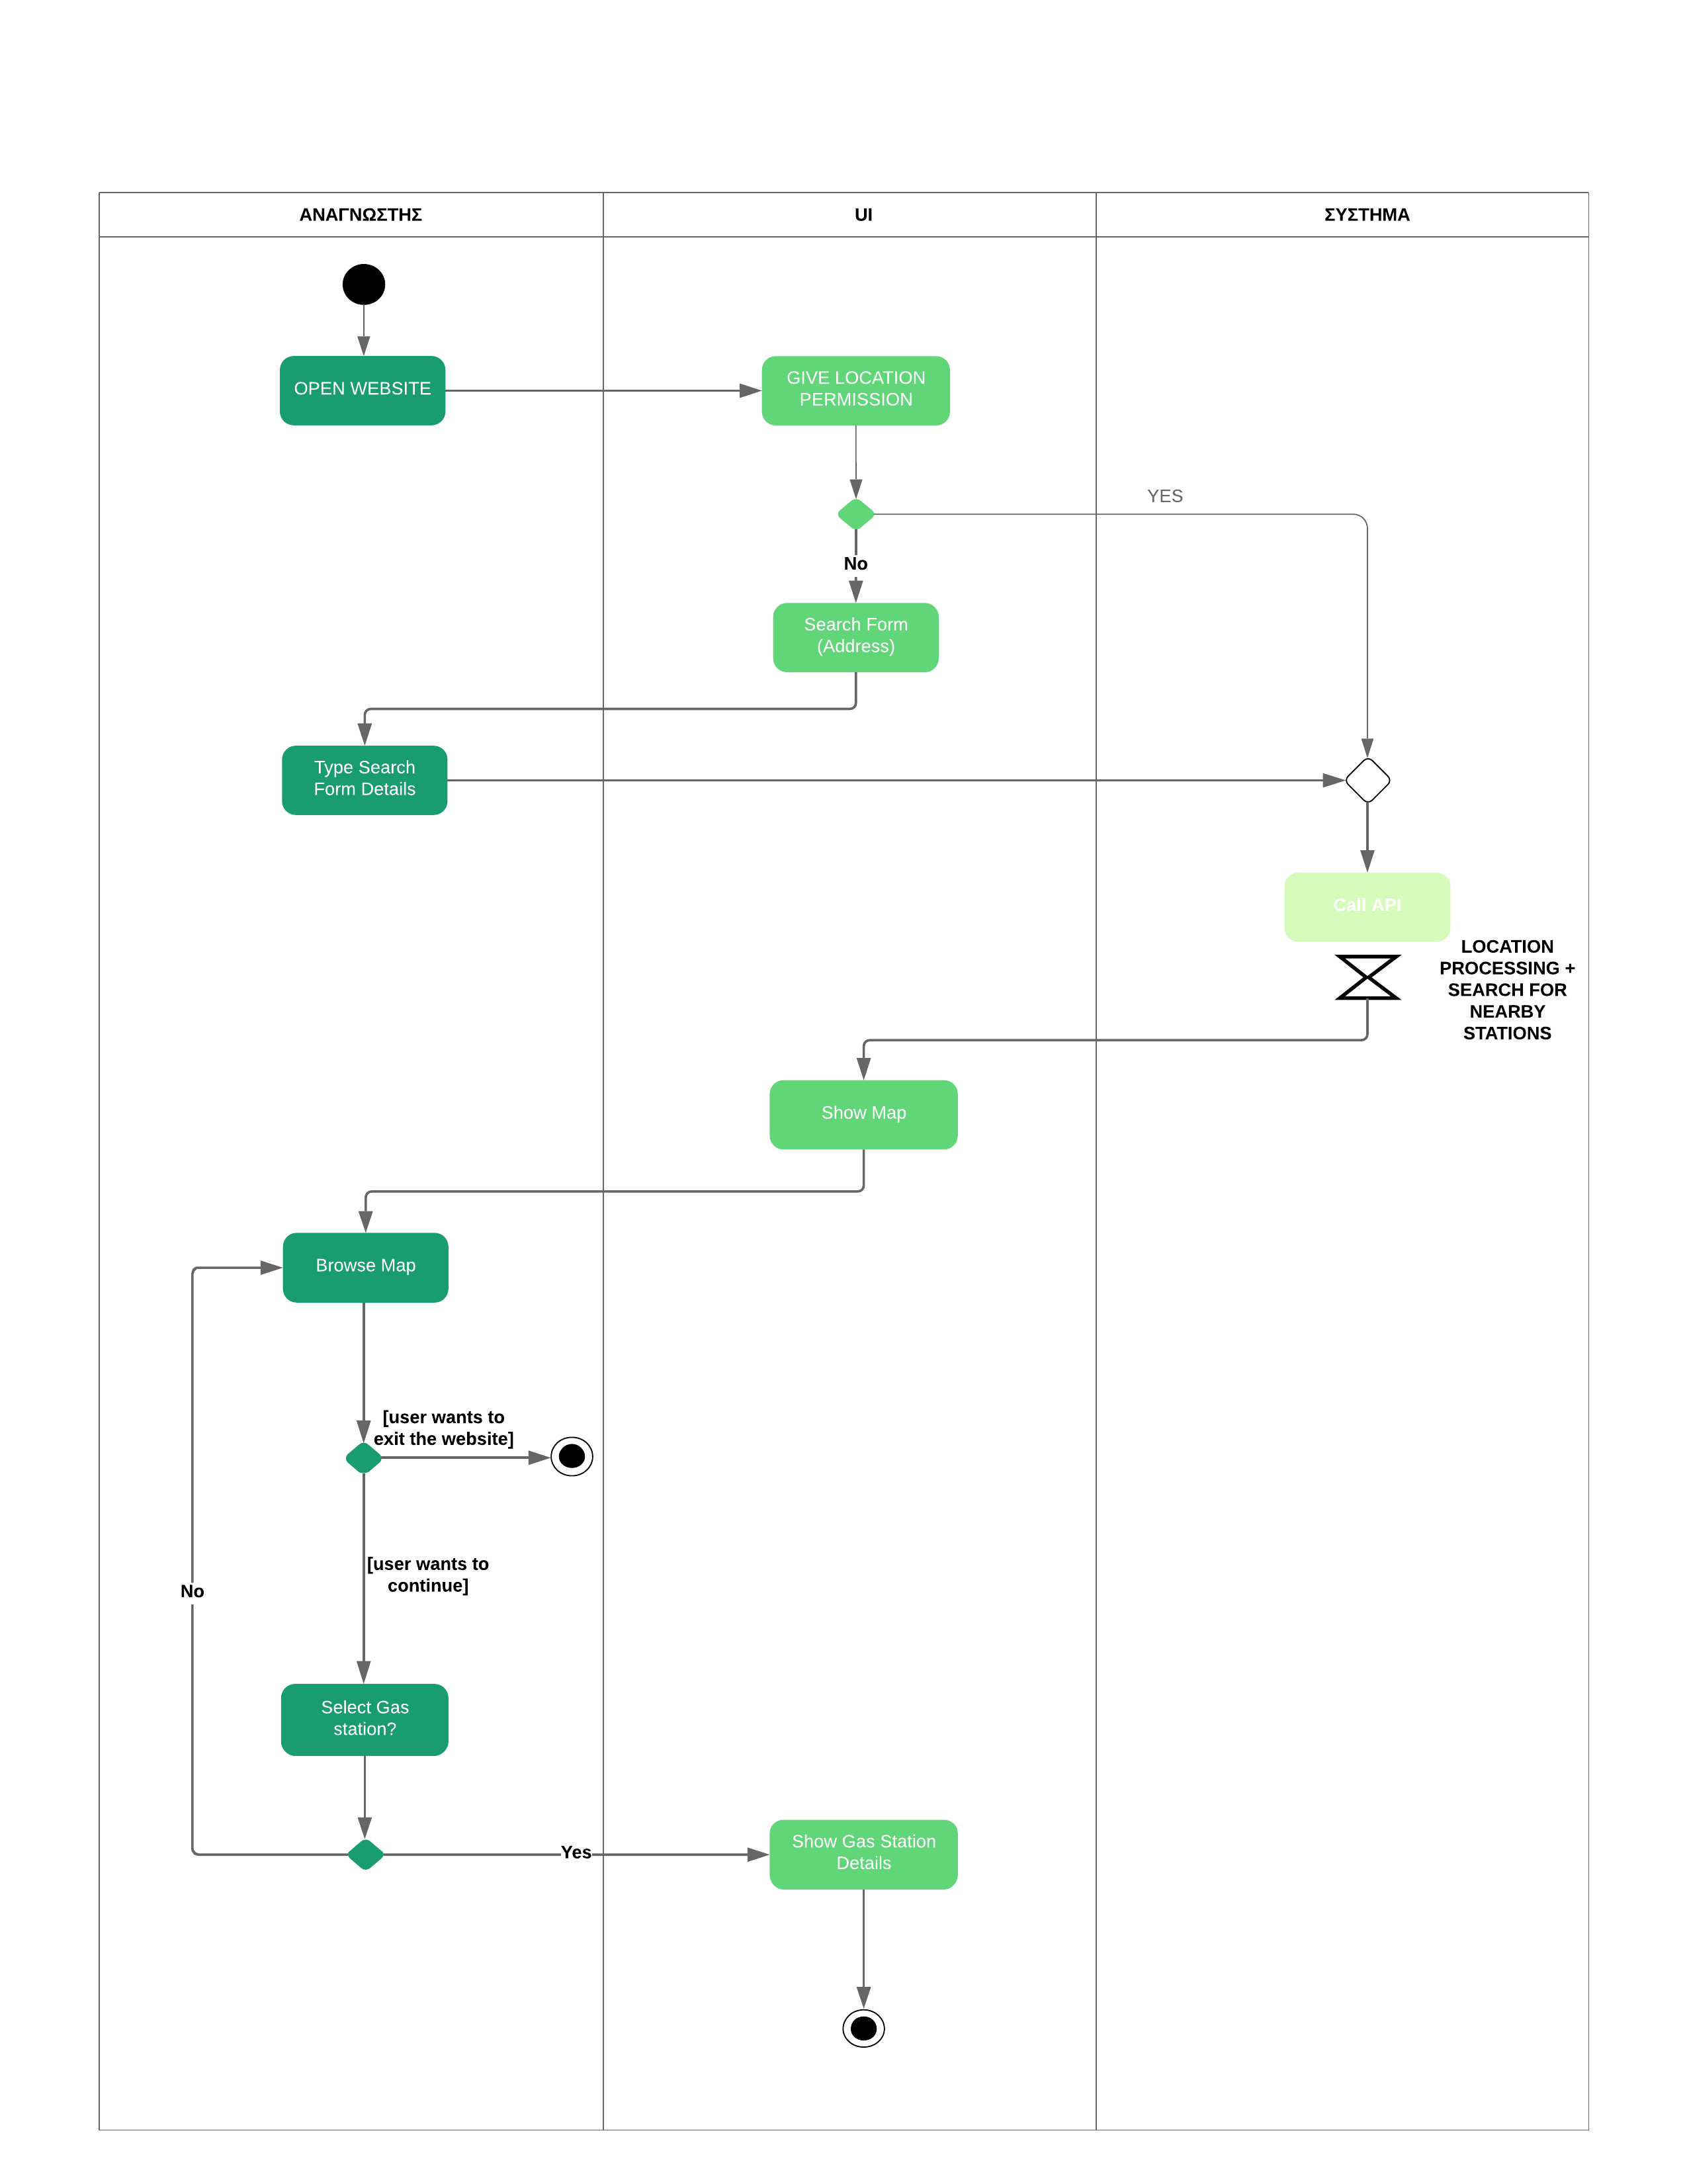
\includegraphics[width = \linewidth]{uml/reader.png}
	\caption{UML activity diagram για \texttt{ΑΝΑΓΝΩΣΤΗ}}
\end{figure}


\subsubsection*{Εθελοντής}

Ο χρήστης εθελοντής πέρα από όλες τις δυνατότητες του χρήστη αναγνώστη έχει τη δυνατότητα να κάνει sign in με βάση τα προσωπικά του στοιχεία. \\
Με τον τρόπο αυτό το σύστημα κάνει retrieve από τη βάση δεδομένων το προφίλ του και επιπλέον λάμβάνει τη γεωγραφική του τοποθεσία (θεωρείται πως με τον τρόπο αυτό δίνει άμεσα τη συγκατάθεσή του) και εμφανίζει την τοποθεσία του στο χάρτη.\\
Επιπρόσθετα, ο εθελοντής έχει τη δυνατότητα να εισάγει κάνοντας insert/update τις πλέον πρόσφατες τιμές για το πρατήριο της επιλογής του.\\
Η παραπάνω συμπεριφορά μοντελοποιείται με το κάτωθι διάγραμμα δραστηριοτήτων UML.
\begin{figure}
	\centering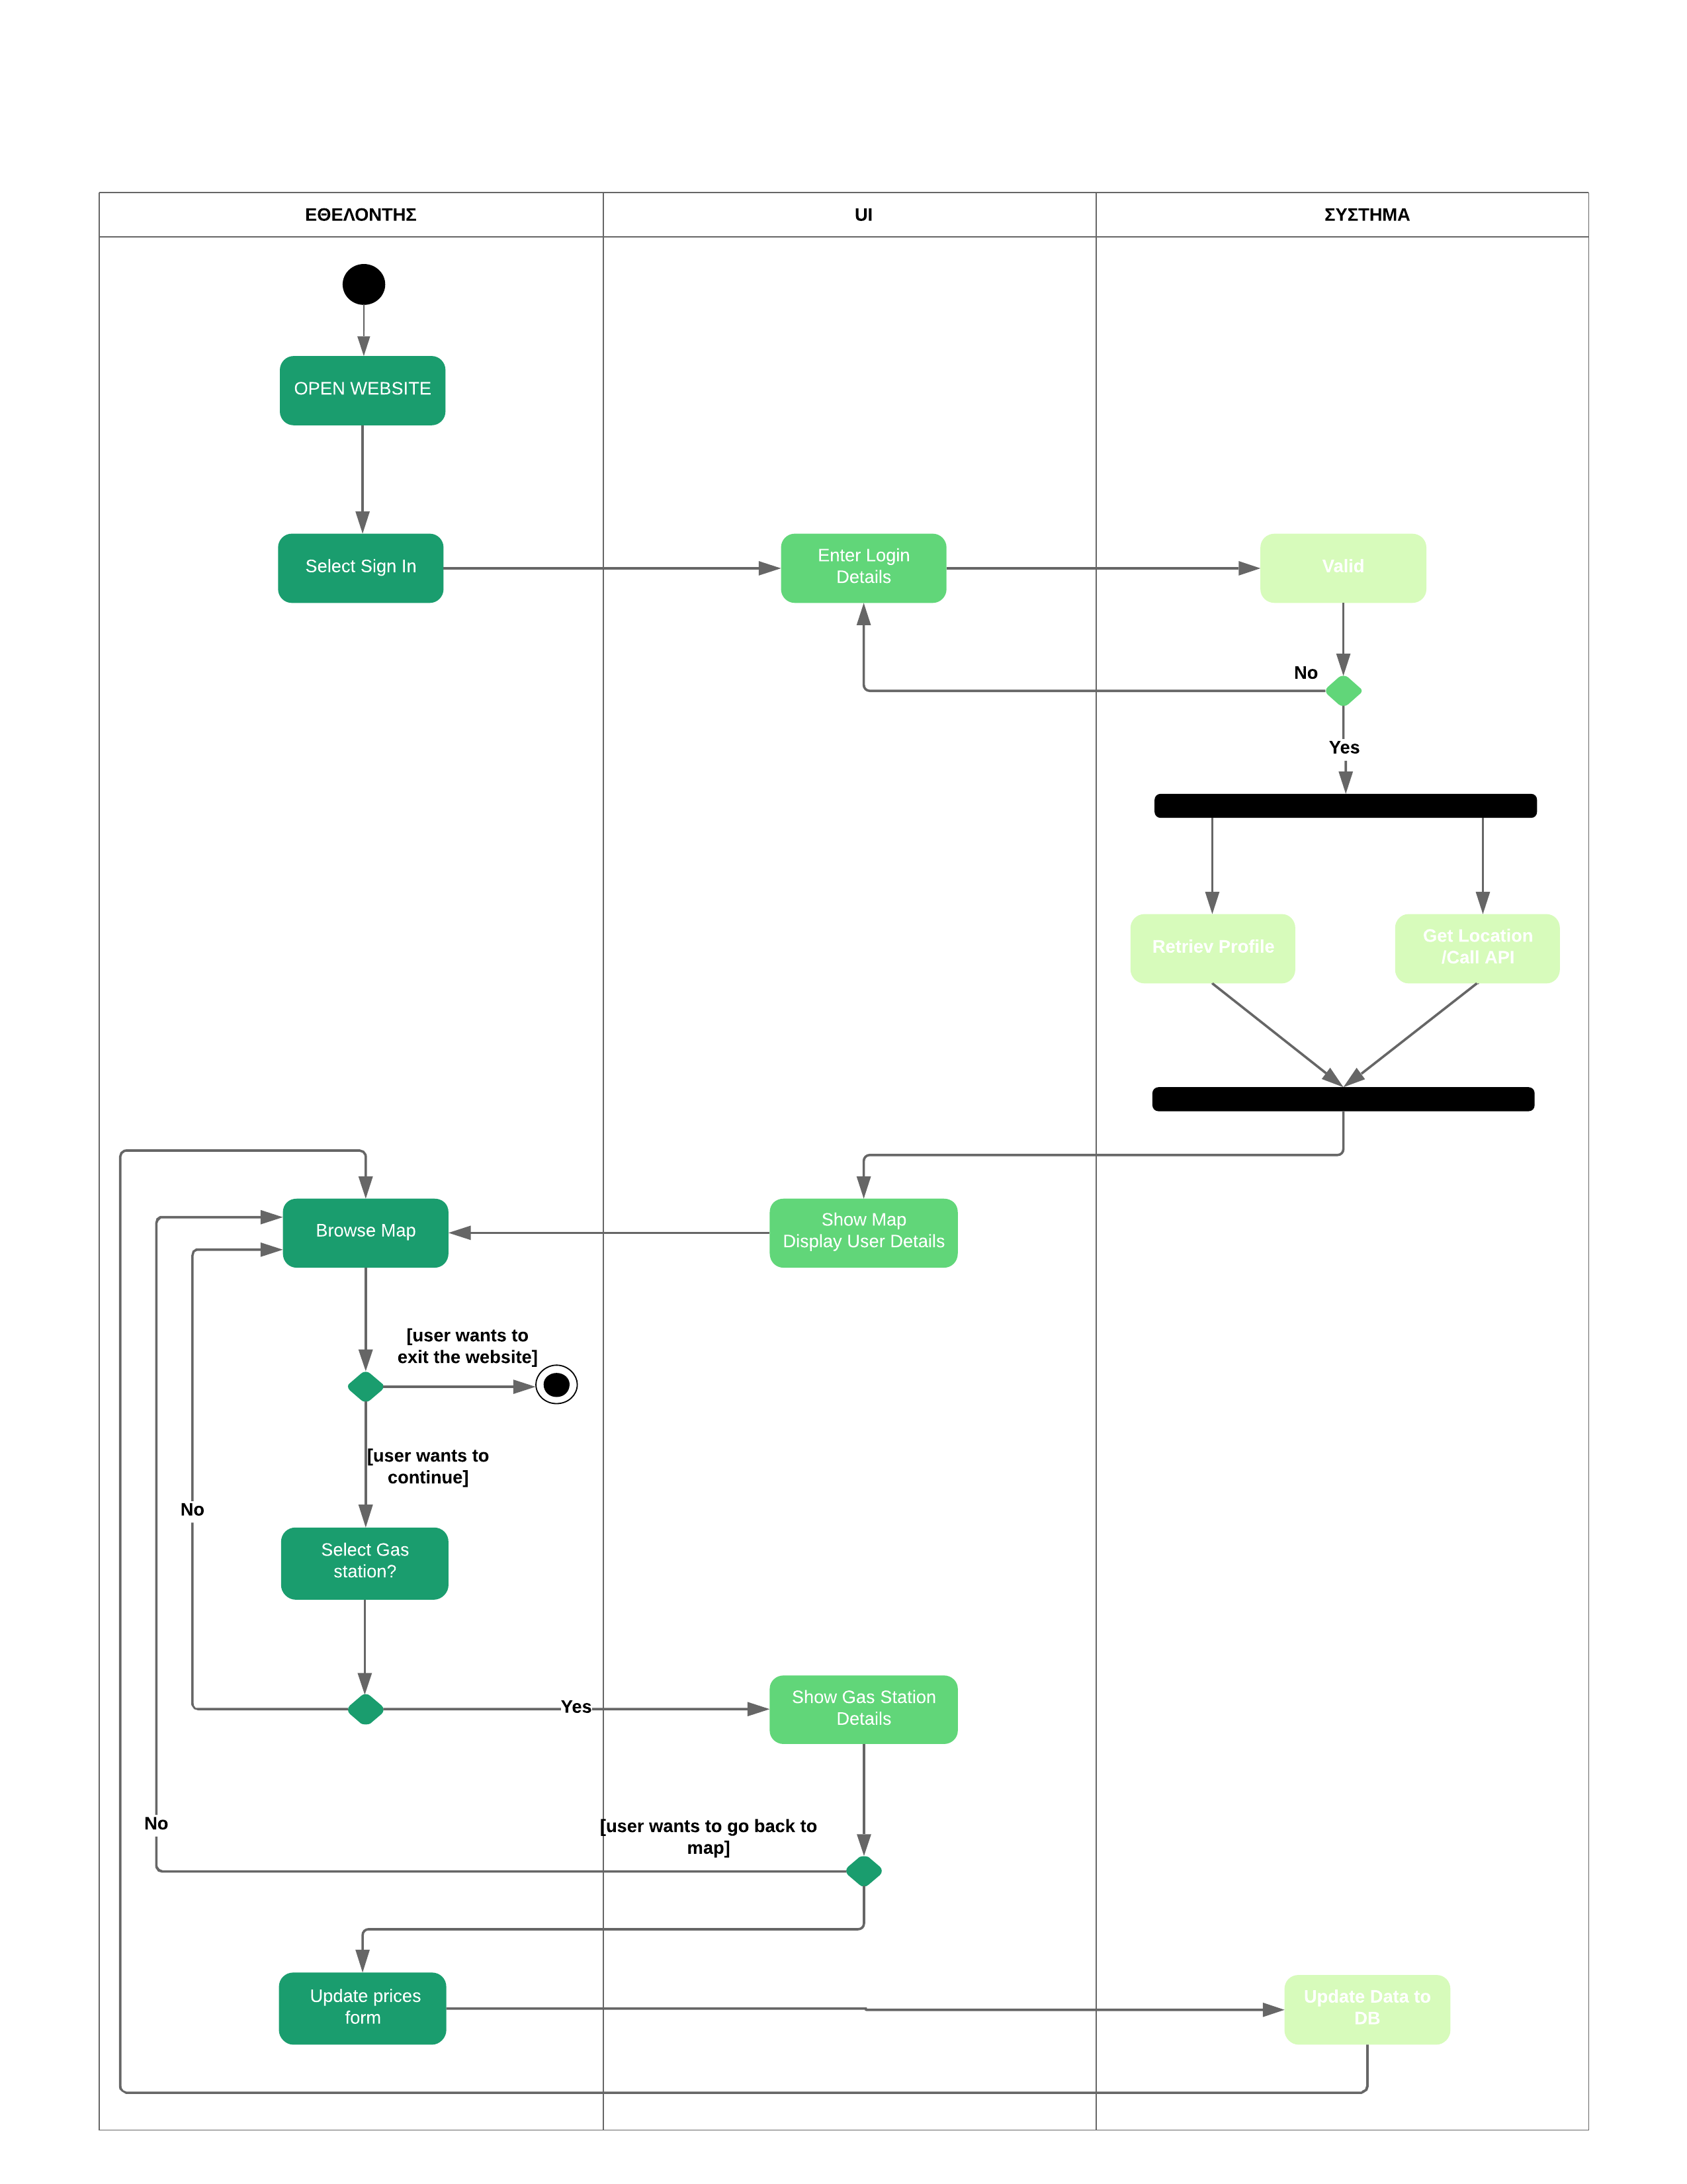
\includegraphics[width = \linewidth]{uml/volunteer.png}
	\caption{UML activity diagram για \texttt{ΕΘΕΛΟΝΤΗ} (εγγεγραμένος χρήστης)}
\end{figure}